\documentclass{report}

\usepackage{array}
\usepackage{amsmath,amssymb,amsfonts,mathrsfs,amsthm}
\usepackage[utf8]{inputenc}
\usepackage{listings}
\usepackage{mathtools}
\usepackage{dsfont}
\usepackage{pdfpages}
\usepackage[textsize=footnotesize,color=green]{todonotes}
\usepackage{algorithm, algorithmic}
\usepackage{bm}
\usepackage{tikz}
\usepackage[normalem]{ulem}

\usepackage{graphicx}
\usepackage{subfigure}
\usepackage{color}
\usepackage{undertilde}
\usepackage[colorlinks = true, filecolor = red, urlcolor = blue, linkcolor = black]{hyperref}
\usepackage{pdflscape}
\usepackage{pifont}
%\usepackage{fullpage}
\setlength\textwidth{6in}
\setlength\textheight{8in}
\setlength\oddsidemargin{0.25in} % LaTeX adds a default 1in to this!
\setlength\evensidemargin{0.25in}
\setlength\topmargin{-0.0in} % LaTeX adds a default 1in to this!
\setlength\headsep{0in}
\setlength\headheight{0in}
\setlength\footskip{1in}

\renewcommand{\topfraction}{0.85}
\renewcommand{\textfraction}{0.1}
\renewcommand{\floatpagefraction}{0.75}

\newcommand{\vect}[1]{\ensuremath\boldsymbol{#1}}
\newcommand{\tensor}[1]{\underline{\vect{#1}}}
\newcommand{\del}{\triangle}
\newcommand{\grad}{\nabla}
\renewcommand{\div}{\grad \cdot}
\newcommand{\ip}[1]{\left\langle #1 \right\rangle}
\newcommand{\eip}[1]{a\left( #1 \right)}
\newcommand{\pd}[2]{\frac{\partial#1}{\partial#2}}
\newcommand{\pdd}[2]{\frac{\partial^2#1}{\partial#2^2}}

\newcommand{\circone}{\ding{192}}
\newcommand{\circtwo}{\ding{193}}
\newcommand{\circthree}{\ding{194}}
\newcommand{\circfour}{\ding{195}}
\newcommand{\circfive}{\ding{196}}

\newcommand{\Reyn}{\rm Re}

\newcommand{\bs}[1]{\boldsymbol{#1}}
\DeclareMathOperator{\diag}{diag}

\newcommand{\equaldef}{\stackrel{\mathrm{def}}{=}}

\newcommand{\tablab}[1]{\label{tab:#1}}
\newcommand{\tabref}[1]{Table~\ref{tab:#1}}

\newcommand{\theolab}[1]{\label{theo:#1}}
\newcommand{\theoref}[1]{\ref{theo:#1}}
\newcommand{\eqnlab}[1]{\label{eq:#1}}
\newcommand{\eqnref}[1]{\eqref{eq:#1}}
\newcommand{\seclab}[1]{\label{sec:#1}}
\newcommand{\secref}[1]{\ref{sec:#1}}
\newcommand{\lemlab}[1]{\label{lem:#1}}
\newcommand{\lemref}[1]{\ref{lem:#1}}

\newcommand{\mb}[1]{\mathbf{#1}}
\newcommand{\mbb}[1]{\mathbb{#1}}
\newcommand{\mc}[1]{\mathcal{#1}}
\newcommand{\nor}[1]{\left\| #1 \right\|}
\newcommand{\snor}[1]{\left| #1 \right|}
\newcommand{\LRp}[1]{\left( #1 \right)}
\newcommand{\LRs}[1]{\left[ #1 \right]}
\newcommand{\LRa}[1]{\left\langle #1 \right\rangle}
\newcommand{\LRc}[1]{\left\{ #1 \right\}}
\newcommand{\tanbui}[2]{\textcolor{blue}{\sout{#1}} \textcolor{red}{#2}}
\newcommand{\Grad} {\ensuremath{\nabla}}
\newcommand{\Div} {\ensuremath{\nabla\cdot}}
\newcommand{\Nel} {\ensuremath{{N^\text{el}}}}
\newcommand{\jump}[1] {\ensuremath{\LRs{\![#1]\!}}}
\newcommand{\uh}{\widehat{u}}
\newcommand{\fnh}{\widehat{f}_n}
\renewcommand{\L}{L^2\LRp{\Omega}}
\newcommand{\pO}{\partial\Omega}
\newcommand{\Gh}{\Gamma_h}
\newcommand{\Gm}{\Gamma_{-}}
\newcommand{\Gp}{\Gamma_{+}}
\newcommand{\Go}{\Gamma_0}
\newcommand{\Oh}{\Omega_h}

\newcommand{\eval}[2][\right]{\relax
  \ifx#1\right\relax \left.\fi#2#1\rvert}

\def\etal{{\it et al.~}}


\def\arr#1#2#3#4{\left[
\begin{array}{cc}
#1 & #2\\
#3 & #4\\
\end{array}
\right]}
\def\vecttwo#1#2{\left[
\begin{array}{c}
#1\\
#2\\
\end{array}
\right]}
\def\vectthree#1#2#3{\left[
\begin{array}{c}
#1\\
#2\\
#3\\
\end{array}
\right]}
\def\vectfour#1#2#3#4{\left[
\begin{array}{c}
#1\\
#2\\
#3\\
#4\\
\end{array}
\right]}
\date{}
\author{Jesse Chan}
\title{Proposal outline/notes}

\newtheorem{proposition}{Proposition}
\newtheorem{corollary}{Corollary}
\newtheorem{theorem}{Theorem}
\newtheorem{lemma}{Lemma}

\begin{document}

\tableofcontents
\maketitle

\chapter{Introduction}

\section{Motivations}

Adaptivity and stability for CFD problems are issues for high Reynolds and Mach numbers. 
\todo{FINISH}

Address the fact that CFD problems have issues of robustness; introduce reasoning that we will study the model problem of convection-diffusion first to better understand this. 

\subsection{Singular perturbation problems and robustness}

Historically, the Galerkin method has been very successfully applied to a broad range of problems in solid mechanics, for which the variational problems resulting from the PDE are symmetric and coercive (positive-definite). It is well known that the finite element method produces optimal or near-optimal results for such problems, with the finite element solution matching or coming close to the best approximation of the solution in the finite element space. However, standard Bubnov-Galerkin methods tend to perform poorly for the class of PDEs known as singular perturbation problems. These problems are often characterized by a parameter that may be either very small or very large in the context of physical problems.  An additional complication of singular perturbation problems is that very often, in the limiting case of the parameter blowing up or decreasing to zero, the PDE itself will change types (e.g.\ from elliptic to hyperbolic).

A canonical example of a singularly perturbed problem is the convection-diffusion equation on domain $\Omega \in \mathbb{R}^3$,
\[
\div \left(\beta u\right) - \epsilon \Delta u = f.
\]
The equation represents the change in the scalar quantity $u$, representing the concentration of a quantity in a given medium, taking into account both convective and diffusive effects. $\beta \in \mathbb{R}^3$ specifies the direction and magnitude of convection, while the singular perturbation parameter $\epsilon$ represents the diffusivity of the medium. In the limit of an inviscid medium as $\epsilon\rightarrow 0$, the equation changes types, from elliptic to hyperbolic, and from second order to first order.

We will illustrate the issues associated with numerical methods for this equation using one dimensional examples.  In 1D, the convection-diffusion equation is
\begin{align*}
\beta u'-\epsilon u'' &= f.
\end{align*}
For Dirichlet boundary conditions $u(0)=u_0$ and $u(1)= u_1$, the solution can develop sharp boundary layers of width $\epsilon$ near the outflow boundary $x=1$. 

\begin{figure}[!h]
\centering
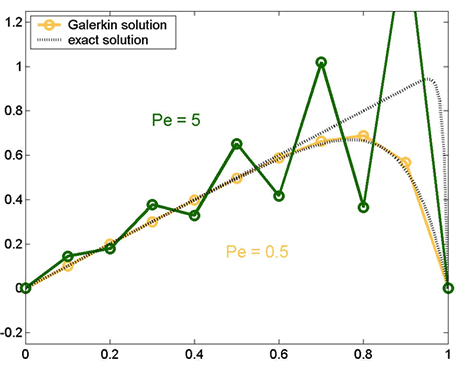
\includegraphics[scale=.4]{figs/GalerkinOscTight.png}
\caption{Oscillations in the 1D finite element solution of the convection-diffusion equation for small diffusion.}
\label{fig:GalerkinOsc}
\end{figure}

The poor performance of the finite element method for this problem is reflected in the bound on the error in the finite element solution --- under the standard Bubnov-Galerkin method with $u\in H^1(0,1)$, we have the bound given in \cite{roos2008robust}:
\[
\|u-u_h\|_\epsilon \leq C \inf_{w_h}\|u-w_h\|_{H^1(0,1)},
\]
for $\|u\|_\epsilon^2 \coloneqq \|u\|_{L^2}^2 + \epsilon \|u'\|_{L^2}^2$, with $C$ independent of $\epsilon$. An alternative formulation of the above bound is 
\[
\|u-u_h\|_{H^1(0,1)} \leq C(\epsilon) \inf_{w_h}\|u-w_h\|_{H^1(0,1)},
\]
where $C(\epsilon)$ grows as $\epsilon\rightarrow 0$. The dependence of the constant $C$ on $\epsilon$ is referred to as a \textit{loss of robustness} --- as the singular perturbation parameter $\epsilon$ decreases, our finite element error is bounded more and more loosely by the best approximation error.  As a consequence, the finite element solution can diverge significantly from the best finite element approximation of the solution for very small values of $\epsilon$.  For example, Figure~\ref{fig:GalerkinOsc} shows an example of how, on a coarse mesh, and for small values of $\epsilon$, the Galerkin approximation of the solution to the convection-diffusion equation with a boundary layer develops spurious oscillations everywhere in the domain, even where the best approximation error is small.  These oscillations grow in magnitude as $\epsilon \rightarrow 0$, eventually polluting the entire solution.  

\section{Goal}

To develop a robust, stable $hp$-adaptive scheme for the steady compressible laminar Navier-Stokes equations in transonic/supersonic regimes.
\todo{FINISH}

\section{Literature review}

For the past half-century, problems in computational fluid dynamics (CFD) have been solved using a multitude of methods, many of which are physically motivated, and thus applicable only to a small number of problems and geometries. We consider more general methods, whose framework is applicable to different problems in CFD; however, our specific focus will be on the nonlinear shock problems of compressible aerodynamics. Broadly speaking, the most popular general methods include (in historical order) finite difference methods, finite volume methods, and finite element methods.  

\subsection{Finite difference and finite volume methods}

For linear problems, finite difference (FD) methods approximate derivatives based on interpolation of pointwise values of a function.  FD methods were popularized first by Lax, who introduced the concepts of the monotone scheme and numerical flux. For the conservation laws governing compressible aerodynamics, FD methods approximated the conservation law, using some numerical flux to reconstruct approximations to the derivative at a point. Finite volume (FV) methods are similar to finite difference methods, but approximate the integral version of a conservation law as opposed to the differential form. FD and FV have roughly the same computational cost/complexity; however, the advantage of FV methods over FD is that FV methods can be used on a much larger class of discretizations than FD methods, which require uniform or smooth meshes. 

For nonlinear shock problems, the solution often exhibits sharp gradients or discontinuities, around which the solution would develop spurious Gibbs-type oscillations. Several ideas were introduced to deal with oscillations in the solution near a sharp gradient or shock: artificial diffusion, total variation diminishing (TVD) schemes, and slope limiters. However, each method had its drawback, either in terms of loss of accuracy, dimensional limitations, or problem-specific parameters to be tuned \cite{Shu:Lectures}. Harten, Enquist, Osher and Chakravarthy introduced the essentially non-oscillatory (ENO) scheme in 1987 \cite{ENO}, which was improved upon with the weighted essentially non-oscillatory (WENO) scheme in \cite{WENO}. WENO remains a popular choice today for both finite volume and finite difference schemes. Most of these methods can be interpreted as adding some specific artificial diffusion to the given numerical scheme.  We refer to such schemes as \emph{modified equation} methods, as the exact solution no longer satisfies the discrete system due to the presence of additional artificial diffusion.  

Historically, finite volumes and finite difference methods have been the numerical discretizations of choice for CFD applications; the simplicity of implementation of the finite difference method allows for quick turnaround time, and the finite volume method is appealing due to its locally conservative nature and flexibility. More recently, the finite element (FE) method has gained popularity as a discretization method for CFD applications for its stability properties and rigorous mathematical foundations. Early pioneers of the finite element method for CFD included Zienkiewicz, Oden, Karniadakis, and Hughes \cite{ChungCFDBook}.  

\subsection{Stabilized finite element methods}

The finite element/Galerkin method has been widely utilized in engineering to solve partial differential equations governing the behavior of physical phenomena in engineering problems.  The method relates the solution of a partial differential equation (PDE) to the solution of a corresponding variational problem. The finite element method itself provides several advantages --- a framework for systematic mathematical analysis of the behavior of the method, weaker regularity constraints on the solution than implied by the strong form of the equations, and applicability to very general physical domains and geometries for arbitrary orders of approximation. 

Traditionally, instability/loss of robustness in finite element methods has been dealt with using residual-based stabilization techniques.  Given some variational form, the problem is modified by adding to the bilinear form the strong form of the residual, weighted by a test function and scaled by a stabilization constant $\tau$.  The most well-known example of this technique is the streamline-upwind Petrov-Galerkin (SUPG) method, which is a stabilized FE method for solving the convection-diffusion equation using piecewise linear continuous finite elements \cite{SUPG}.  SUPG stabilization not only removes the spurious oscillations from the finite element solution of the convection-diffusion equation, but delivers the best finite element approximation in the $H^1$ norm.  

\subsubsection{SUPG}

The Streamline Upwind Petrov Galerkin (SUPG) method is a stabilization method for $H^1$-conforming finite elements, the idea of which was originally motivated by artificial diffusion techniques in finite differences.  In particular, for the homogeneous 1D convection-diffusion equation, it is possible to recover, under a finite difference method, the exact solution at nodal points by adding an ``exact" artificial diffusion based on the mesh size $h$ and the magnitudes of the convection $\beta$ and the viscosity $\epsilon$.  

The idea of ``exact" artificial viscosity was adapted to finite elements not through the direct modification of the equations, but through the test functions and weighting of the residual.  In particular, finite element and Galerkin methods are often referred to as ``weighted residual" methods, since the starting point of both is to multiply the residual by a particular test, or weighting, function.  Standard Galerkin methods, known as Bubnov-Galerkin methods, simply choose these weighting functions to be the same as the the basis functions used to approximate the solution.  A Petrov-Galerkin method refers to any Galerkin method other than a classical Bubnov-Galerkin method.  

We will introduce the SUPG method at an abstract level for illustrative purposes only.  Further details and perspectives on the SUPG method can be found in \cite{SUPG}, as well as in an upcoming book by Hughes.  The convection-diffusion equation can be written as follows:
\[
Lu = \left(L_{\rm adv} + L_{\rm diff} \right) u = f,
\]
where $L_{\rm adv}u \coloneqq \div \left(\beta u\right)$ is the first order advective operator, and $L_{\rm diff}u \coloneqq \epsilon \Delta u$ is the second-order diffusive operator (then, roughly speaking, $L_{\rm diff} u = 0$).  Let us assume $u$ to be a linear combination of piecewise-linear basis functions $\phi_i, i = 0,\ldots,N$.  The SUPG method is then to solve
\[
\int_\Omega L u v + \int_\Omega \tau \left(L_{\rm adv}v\right)\left( L u - f\right) = \int_\Omega f v 
\]
for where $\tau$ is the SUPG parameter.  For uniform meshes in 1D, $\tau$ is chosen such that, for $f=0$, the matrix system resulting from SUPG is exactly equal to the finite difference system under ``exact" artificial diffusion.  However, unlike the artificial diffusion method, for $f\neq 0$, the SUPG method still delivers optimal stabilization.  In fact, the SUPG finite element solution in 1D is nothing less than the nodal interpolant and the best $H^1$ approximation of the exact solution, as seen in Figure~\ref{fig:SUPG}.

\begin{figure}[!h]
\centering
\subfigure[SUPG and standard FEM solutions]{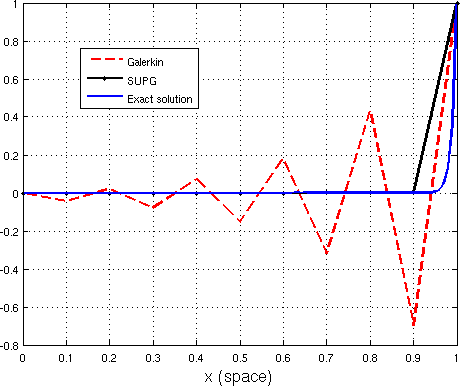
\includegraphics[scale=.43]{figs/SUPG.png}}
\subfigure[SUPG test function]{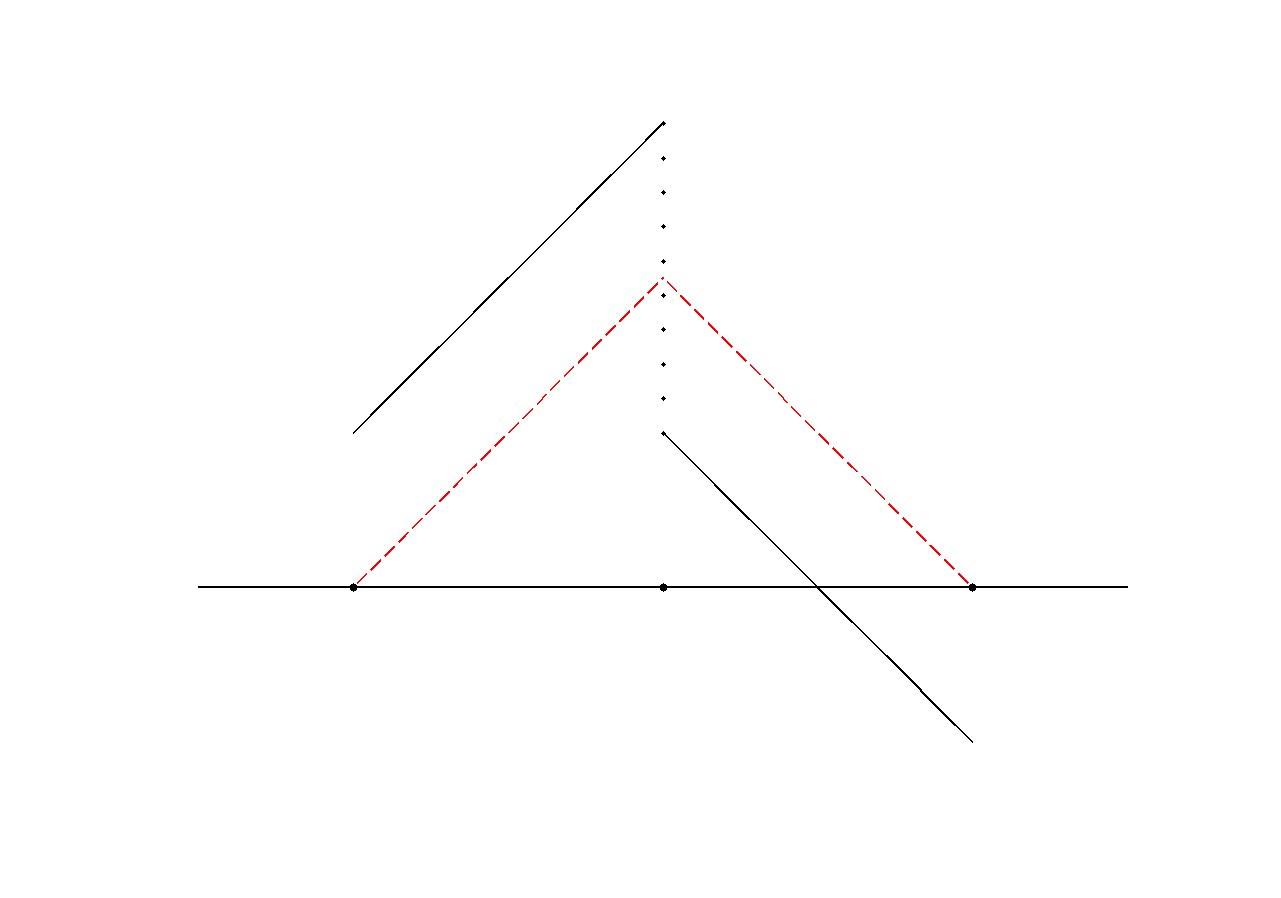
\includegraphics[scale=.22]{figs/SUPGtest.png}}
\caption{SUPG and standard Bubnov-Galerkin solutions to the 1D convection-dominated diffusion equation, and a modified SUPG test function (in black) corresponding to a linear basis ``hat" function (in red).  The upwind portion of the element is emphasized, while the downwind portion is decreased.  The magnitude of the discontinuity between the upwind and downwind portion is controlled by the intrinsic timescale parameter $\tau$. }
\label{fig:SUPG}
\end{figure}

The idea of emphasizing the upwind portion of a test function is an old idea, introduced in 1977 by Zienkiewicz et al.\ in \cite{zienkUpwind}.  However, the precise amount of upwinding,\footnote{Insufficient upwinding results in a method which still exhibits oscillations and instabilities, while excessive upwinding leads to an overly diffusive method.} as well as the connection to residual-based stabilization methods, were novel to SUPG.  

The method can be made to ``work" for $p>1$, but the results are not as strong as for linear elements, and there is no clear generalization of SUPG to higher order elements.  Additionally, the stabilization properties of SUPG are weaker in higher dimensions, and the SUPG solution is no longer the $H^1$ best approximation for 2D and 3D problems \todo{find citation}.  Despite these caveats, SUPG is still the most popular stabilization method of choice for convection-diffusion type problems, in both academic and industry applications.  

An important feature of SUPG and other residual-based stabilization techniques that separates it from modified equation methods is the idea of \textit{consistency} --- by adding stabilization terms based on the residual, the exact solution still satisfies the same variational problem (i.e.\ Galerkin orthogonality still holds). Contrast this to the artificial diffusion methods in finite difference and finite volume methods, where a specific amount of additional viscosity is added based on the magnitude of the convection and diffusion parameters: unlike residual-based stabilization schemes, the exact solution to the original equation no longer satisfies the new stabilized formulation.  

This addition of residual-based stabilization terms can be interpreted as a modification of the test functions as well.  For SUPG, the formulation can equivalently be written as
\[
\int_\Omega\left( Lu-f\right) v_i = \int_\Omega f v_i, \quad i = 0,\ldots,N
\]
where $v_i$ is defined as
\[
v_i = \phi_i(x) + \tau L_{\rm adv} \phi_i.  
\]
In other words, the test function $v_i$ is a perturbation of the basis function $\phi_i$ by a scaled advective operator applied to $\phi_i$.  For a linear $C^0$ basis function (the ``hat" function), this naturally leads to a bias in the upwind or streamline direction of the flow $\beta$, as seen in Figure~\ref{fig:SUPG}.  

An important connection can now be made --- stabilization can be achieved by changing the test space for a given problem.  We will discuss in Section~\secref{optimalTest} approaching the idea of stabilization through the construction of \textit{optimal test functions} to achieve optimal approximation properties. 

\subsubsection{DG methods}

Discontinuous Galerkin (DG) methods form a subclass of FEM; first introduced by Reed and Hill in \cite{Reed:73}, these methods were later analyzed by Cockburn and Shu \cite{CockburnShu:DG} and have rapidly gained popularity for CFD problems. Rather than having a continuous basis where the basis function support spans several element cells, DG opts instead for a discontinuous, piecewise polynomial basis, where, like FV schemes, a numerical flux facilitates communication between neighboring elements (unlike FV methods, however, there is no need for a reconstruction step). Advantages of DG methods include the local conservation property, easily modified local orders of approximation, easy adaptivity in both $h$ and $p$, and efficient parallelizability. 

An additional reason for the popularity of DG methods is that they can be interpreted as stabilized FE methods through appropriate choices of the numerical flux \todo{add Brezzi citation}. We will illustrate this with the pure convection equation in 1D.  

Local conservation: in 1D, numerical solution at outflow is exact.

\todo{Add 1D description and diagrams (Hughes book) of DG formulation for convection with upwind flux.}

For example, for the pure convection problem, the solution has only regularity in the streamline direction, but is only $L^2$ in the crosswind direction. As a consequence, the boundary trace of the solution is defined only in the direction of convection. The upwind DG method addresses the above issue by choosing the numerical flux to be the upwind flux; in this case, the DG numerical flux can be viewed as imparting additional regularity than is present in the solution \cite{DPG1,DPG3}. 

A more recent development in DG methods is the idea of \emph{hybridized} DG (HDG), introduced by Gopalakrishnan and Lazarov \cite{hybridDG}. The hybridized DG framework addresses several criticisms of common DG methods (globally coupled degrees of freedom, complicated/inefficient implementation procedures, suboptimal convergence of approximate fluxes) by identifying degrees of freedom with support only on element edges. Neighboring elements are coupled together only through these degrees of freedom, which can be interpreted as Lagrange multipliers enforcing weak continuity of the trial space. Additionally, HDG methods \todo{add bit about numerical fluxes still used, stabilization param}

\subsubsection{Optimization/NL solvers}

Reference (MIT, Fidkowski)

\todo{Find more nonlinear solvers}

\section{Scope}

This proposal will
\begin{enumerate}
\item Introduce DPG
\item Cover the problem of robustness for model problems
\item Extend results/formulations to nonlinear problems
\item Discuss proposed work
\end{enumerate}

\chapter{Range of CFD problems}

\begin{figure}[!h]
\centering
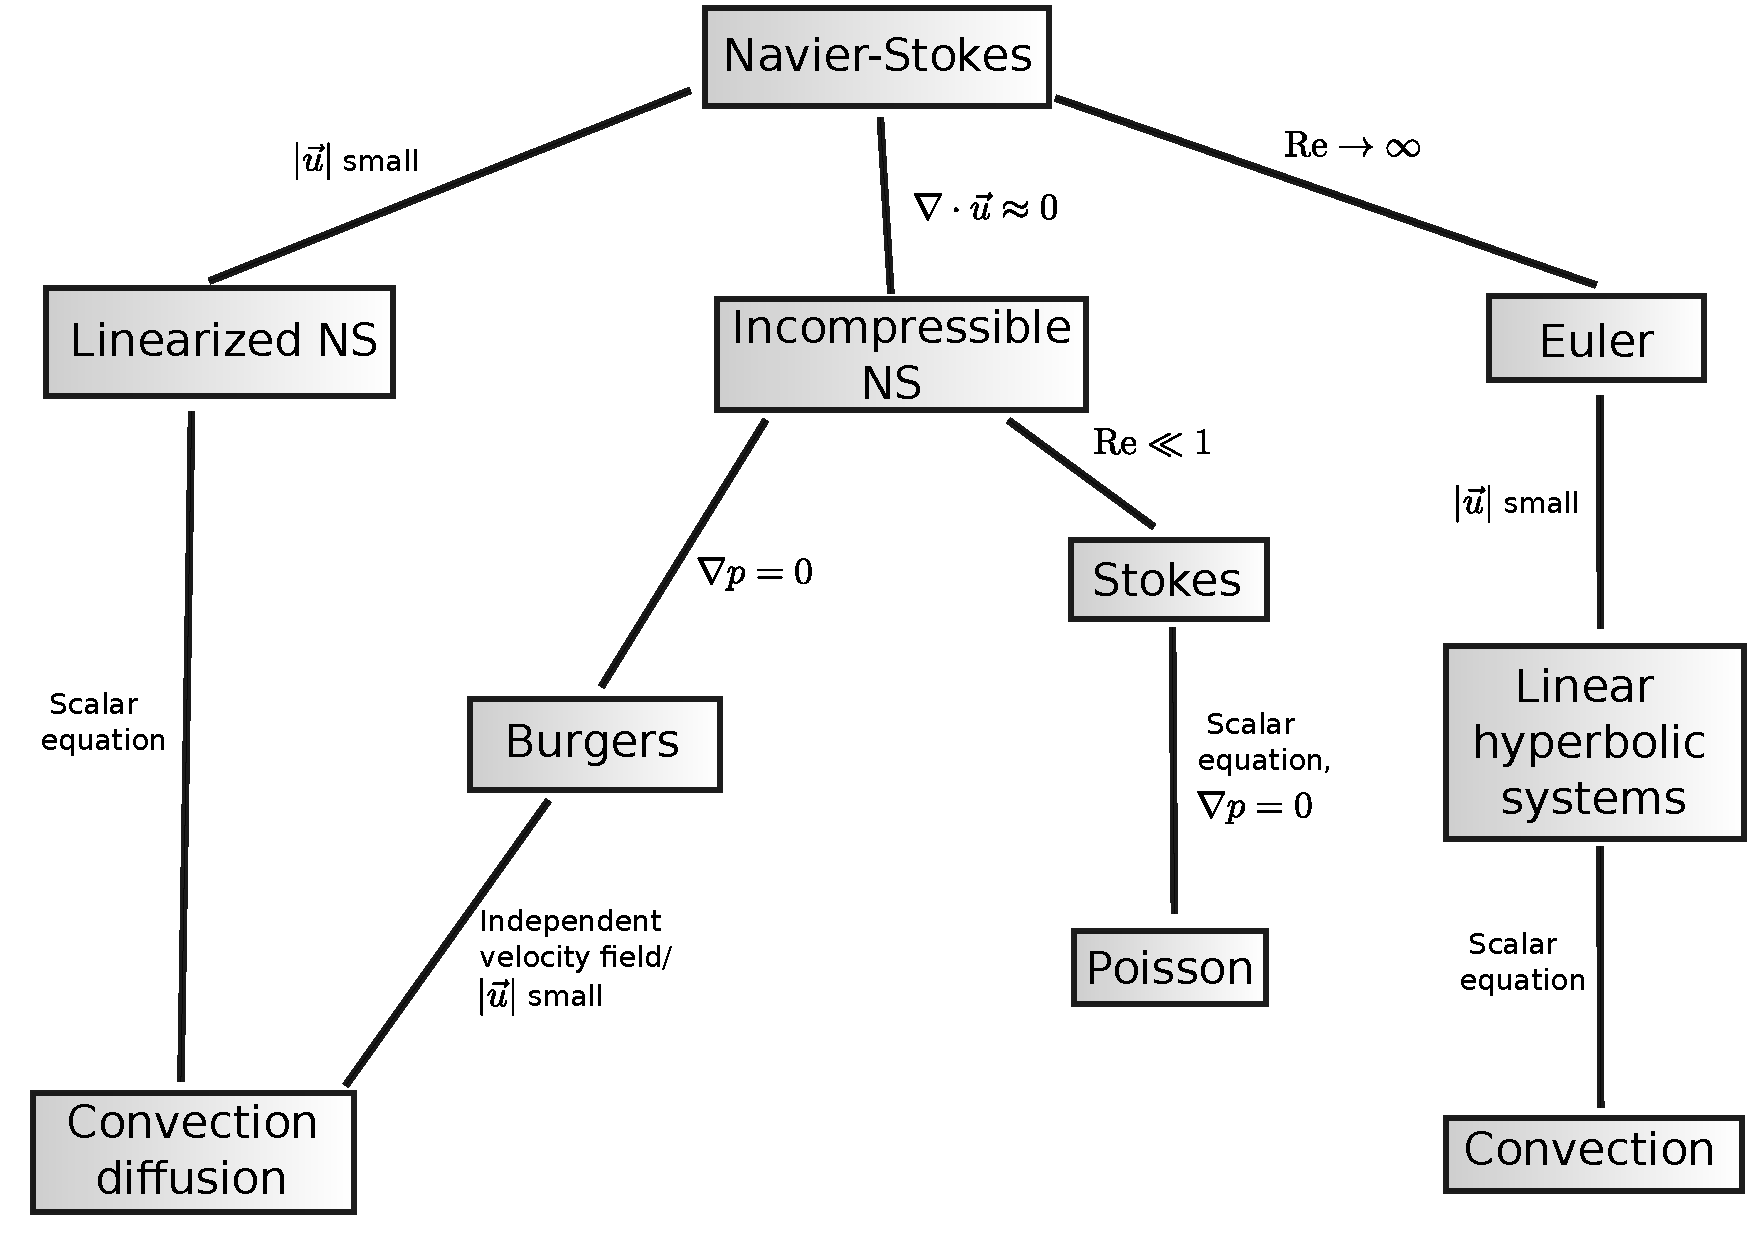
\includegraphics[scale=.45]{figs/CFD_tree.pdf}
\caption{A diagram of common CFD problems and their simplifying assumptions.}
\end{figure}

\begin{itemize}
\item Discuss full compressible Navier-Stokes with boundary layers
\item Discuss full compressible Navier-Stokes without boundary layers, connect to Euler (mention Dr Young and Boeing and the IBL connection \cite{BoeingDrela})
\item Discuss model problems
\end{itemize}

\chapter{Discontinuous Petrov-Galerkin: a minimum residual method for linear problems}

The Discontinuous Petrov-Galerkin (DPG) method of Demkowicz and Gopalakrishnan was first formulated in \cite{DPG1} for the pure convection problem. 

Historically, the name DPG was given by Bottasso, Micheletti, Sacco and Causin to their method for elliptic problems in \cite{BottassoMichelettiSacco02}. The method was then extended to other problems, including convection-diffusion, in \cite{BottassoMichelettiSacco05,CausinSacco05,CausinSaccoBottasso05}. 

The key point in the method of Bottasso et al.\ was their method of hybridization of fluxes. Whereas HDG methods will identify an additional flux unknown on the boundary, the numerical flux coupling neighboring elements together is still typically computed in part using contributions from the field variables. In the DPG formulation, all numerical fluxes are declared to be independent unknowns, leaving the interior field degrees of freedom completely uncoupled from element to element. \todo{Finish, check if this is true.}

The breakthrough came in \cite{DPG2}, where the concept of locally-computable optimal test functions led to the development of the DPG method in its current form.

\todo{Clean up}
This DPG method with optimal test functions is better understood in \cite{DPG3,DPG4}, extended to problems in \cite{DPGElas,stokesDPG}, well-posedness theory developed for Poisson and convection-diffusion in \cite{analysisDPG}, extended to large class of Friedrichs systems in \cite{Bui-ThanhDemkowiczGhattas11b}. \cite{practicalDPG}. 

Optimal order comparison to DG in \cite{DPG1}. Comparisons to other DG methods in \cite{Bui-ThanhDemkowiczGhattas11a,DGDPG}.

\section{Optimal Petrov-Galerkin methods}

\seclab{optimalTest} Petrov-Galerkin methods, in which the test space differs from the trial space, have been explored for over 30 years, beginning with the approximate symmetrization method of Barrett and
Morton~\cite{BARRETT01101981}. The idea was continued with the SUPG method of Hughes, and the characteristic Petrov-Galerkin approach of Demkowicz and Oden~\cite{Demkowicz1986188}, which introduced the
idea of tailoring the test space to change the norm in which a finite element method would converge.

The idea of optimal test functions was introduced by Demkowicz and Gopalakrishnan in \cite{DPG2}.  Conceptually, these optimal test functions are the natural result of the minimization of a residual corresponding to the operator form of a variational equation. The connection between stabilization and least squares/minimum residual methods has been observed previously \cite{GLS}. However, the method in \cite{DPG2} distinguishes itself by measuring the residual of the natural \textit{operator form of the equation}, which is posed in the dual space, and measured with the dual norm, as we now discuss. 	

Throughout the paper, we assume that the trial space $U$ and test space $V$ are real Hilbert spaces, and denote $U'$ and $V'$ as the respective topological dual spaces. Let $U_h \subset U$ and $V_h\subset V$ be finite dimensional subsets. We are interested in the following problem  
\begin{equation}
\eqnlab{variationEq}
\left\{
  \begin{array}{l}
    \text{Given } l \in V', \text{ find } u_h \in U_h  \text{ such that} \\ 
    b(u_h,v_h) = l(v_h), \quad \forall v_h\in V_h,
  \end{array}
  \right.
\end{equation}
where $b\LRp{\cdot,\cdot}: U \times V \to \mbb{R}$ is a continuous
bilinear form.  $U$ is chosen to be some trial space of approximating functions, but $V_h$ is as of yet unspecified. 

Throughout the paper, we suppose the variational
problem \eqnref{variationEq} to be well-posed. In that case, we can
identify a unique operator $B:U\rightarrow V'$ such that
\[
\langle Bu,v\rangle_V \coloneqq b(u,v), \quad u\in U, v\in V
\]
with $\LRa{\cdot, \cdot}_V$ denoting the duality pairing between $V'$ and $V$, to obtain the operator form of the continuous variational problem
\begin{equation}
\eqnlab{dualEq}
Bu = l \quad \text{in } V'.
\end{equation}
In other words, we can represent the continuous form of our variational equation
\eqnref{variationEq} equivalently as the operator equation \eqnref{dualEq} with values in the
dual space $V'$.  This motivates us to consider the conditions under which the solution to \eqnref{variationEq} is the solution to the minimum residual problem in $V'$ 
\[
u_h = \underset{u_h\in U_h}{\arg\min}\, J(u_h),
\]
where $J(w)$ is defined for $w\in U$ as 
\[
J(w) = \frac{1}{2}\|Bw-l\|_{V'}^2 \coloneqq\frac{1}{2} \sup_{v\in V\setminus\{0\}} \frac{| b(w,v)-l(v)|^2}{\nor{v}_V^2}.
\]
For convenience in writing, we will abuse the notation $\sup_{v \in V}$ to denote $\sup_{v\in V\setminus\{0\}}$ for the remainder of the paper.

Let us define $R_V: V \to V'$ as the Riesz map, which identifies
elements of $V$ with elements of $V'$ by 
\[
\langle R_V v,\delta
v\rangle_V \coloneqq(v, \delta v)_V, \quad \forall \delta v \in V.
\]
Here, $(\cdot, \cdot)_V$ denotes the
inner product in $V$. As $R_V$ and its inverse, $R_V^{-1}$, are both
isometries, e.g.\ $\|f\|_{V'} = \|R_V^{-1} f\|_V, \forall f \in V'$, we
have
\begin{equation}
\eqnlab{minimization}
\min_{u_h\in U_h} J(u_h) = \frac{1}{2}\left\|Bu_h-l\right\|_{V'}^2 =  \frac{1}{2}\left\|R_V^{-1}(Bu_h-l)\right\|_V^2.
\end{equation}
The first order optimality condition for \eqnref{minimization} requires
the G\^ateaux derivative to be zero in all directions $\delta u \in
U_h$, i\.e\.,
\begin{align*}
\left(R_V^{-1}(Bu_h-l),R_V^{-1}B\delta u\right)_V = 0, \quad \forall \delta u \in U. 
\end{align*}
We define, for a given $\delta u \in U$, the corresponding {\em optimal test function} $v_{\delta u}$
\begin{equation}
\eqnlab{optv}
v_{\delta u} \coloneqq R_V^{-1}B\delta u \quad  \text{in } V.
\end{equation} 
The optimality condition then becomes
\[
 \langle Bu_h-l, v_{\delta u}\rangle_V = 0, \quad \forall \delta u \in U
\]
which is exactly the standard variational equation in
 \eqnref{variationEq} with $v_{\delta u}$ as the test functions. We can define the optimal test space $V_{\rm opt} \coloneqq \{v_{\delta u} \text{ s.t. } \delta u\in U\}$. Thus, the solution of the variational problem \eqnref{variationEq} with test space $V_h = V_{\rm opt}$ minimizes the residual in the dual norm $\nor{Bu_h-l}_{V'}$. This is the key idea behind the concept of optimal test functions. 

Since $U_h \subset U$ is spanned by a finite number of basis functions $\LRc{\varphi_i}_{i=1}^N$, \eqnref{optv} allows us to compute (for each basis function) a corresponding optimal test function $v_{\varphi_i}$. The collection $\LRc{v_{\varphi_i}}_{i = 1}^N$ of optimal test functions then forms a basis for the optimal test space.  In order to express optimal test functions defined in \eqnref{optv} in a more familiar form, we take  $\delta u = \varphi$, a generic basis function in $U_h$, and rewrite \eqnref{optv} as
\[
R_Vv_{\varphi} = B\varphi, \quad \text{in } V',
\]
which is, by definition, equivalent to
\[
\LRp{v_\varphi,\delta v}_V = \LRa{R_Vv_\varphi,\delta v}_{V}=
\LRa{B\varphi, \delta v}_V = b\LRp{\varphi,\delta v}, \quad
\forall \delta v \in V.
\]
%% Now, let us define the \textit{trial-to-test} operator $T =
%% R_V^{-1}B$, which, by \eqnref{optv}, maps a trial function $\delta u$
%% to its corresponding \textit{optimal} test function $v = T\delta u$.
%% On the other hand,
As a result, optimal test functions can be determined by solving the auxiliary
variational problem
\begin{equation}
\eqnlab{optvVar}
\left(v_\varphi,\delta v\right)_V = b(\varphi,\delta v), \quad \forall
\delta v \in V.
\end{equation}
However, in general, for standard $H^1$ and $H({\rm div})$-conforming finite element methods, test functions are continuous over the entire domain, and hence solving variational problem \eqnref{optvVar} for each optimal test function requires a global operation over the entire mesh, rendering the method impractical. A breakthrough came through the development of
discontinous Galerkin (DG) methods, for which basis functions are
discontinuous over elements. In particular, the use of discontinuous
test functions $\delta v$ reduces the problem of determining global 
optimal test functions
in \eqnref{optvVar} to local problems that can be solved in an
element-by-element fashion.

We note that solving \eqnref{optvVar} on each element exactly is
infeasible since it amounts to inverting the Riesz map $R_V$ exactly.
Instead, optimal test functions are approximated using the standard
Bubnov-Galerkin method on an ``enriched" subspace $\tilde{V} \subset
V$ such that $\dim(\tilde{V}) > \dim(U_h)$ elementwise \cite{DPG1, DPG2}. In this
paper, we assume the error in approximating the optimal test functions
is negligible, and refer to the work in \cite{practicalDPG} for
estimating the effects of approximation error on the performance of DPG.

It is now well known that the DPG method
delivers the best approximation error in the ``energy norm" --- that is
\cite{Bui-ThanhDemkowiczGhattas11a, DPG2,DPG4} 
\begin{equation}
\eqnlab{optimalError}
\nor{u-u_h}_{U,E} = \inf_{w\in U_h} \nor{u-w}_{U,E},
\end{equation}
where the energy norm $\|\cdot \|_{U,E}$ is defined for a function $\varphi \in U$ as
\begin{equation}
\eqnlab{energyNorm} \|\varphi\|_{U,E} \coloneqq \sup_{v\in V}
\frac{b(\varphi,v)}{\|v\|_V} = \sup_{\nor{v}_V = 1} b(\varphi,v) =
\sup_{\nor{v}_V = 1} \LRa{B\varphi,v}_V = \nor{B\varphi}_{V'} =
\nor{v_\varphi}_V,
\end{equation}
where the last equality holds due to the isometry of the Riesz map
$R_V$ (or directly from \eqnref{optvVar} by taking the supremum). An
additional consequence of adopting such an energy norm is that,
without knowing the exact solution, the energy error $\|u-u_h\|_{U,E}$ can
be determined by computing $\|v_{u-u_h}\|_V$ from the following
identity
\[
\left(v_{u-u_h},\delta v\right)_V = b(u-u_h,\delta v) = l\LRp{\delta
v} - b(u_h,\delta v).
\]
This is simply a consequence of the least-squares nature of DPG; the energy error is simply the norm of the  residual in $V'$. 

Practically speaking, this implies that the DPG method is discretely stable on any mesh. In particular, DPG is unconditionally stable for higher order adaptive meshes, where discrete stability is often an issue. 

\section{Ultra-weak variational formulation}
\seclab{abstractUweak}

The naming of the discontinuous Petrov-Galerkin method refers to the fact that the method is a Petrov-Galerkin method, and that the test functions are specified to be discontinuous across element boundaries. There is no specification of the regularity of the trial space, and we stress that the idea of DPG is not inherently tied to a single variational formulation \cite{Bui-ThanhDemkowiczGhattas11a}. 

In most of the DPG literature, however, the discontinuous Petrov-Galerkin method refers to the combination of the concept of locally computable optimal test functions in Section \secref{optimalTest} with the so-called ``ultra-weak formulation" \cite{DPG1,DPG2,DPG3,DPG4,DPGElas,DBLP:journals/procedia/NiemiCC11}. Unlike the previous two sections in which we studied the general equation \eqnref{variationEq} given by abstract bilinear and linear forms, we now consider a concrete instance of \eqnref{variationEq} resulting from an ultra-weak formulation for an abstract first-order system of PDEs $Au = f$. Additionally, from this section onwards, we will refer to DPG as the pairing of the ultra-weak variational formulation with the concept of locally computable optimal test functions. 

We begin by partitioning the domain of interest $\Omega$ into $\Nel$ non-overlapping elements $K_j, j = 1,\hdots,\Nel$ such that $\Oh = \cup_{j=1}^\Nel K_j$ and $\overline{\Omega} = \overline{\Omega}_h$. Here, $h$ is defined as $h= \max_{j\in \LRc{1,\hdots,\Nel}}\text{diam}\LRp{K_j}$.  We denote the mesh ``skeleton" by $\Gh = \cup_{j=1}^\Nel \partial K_j$; the set of all faces/edges $e$, each of which comes with a normal vector ${n}_e$. The internal skeleton is then defined as $\Gamma^0_h = \Gh \setminus \partial \Omega$. If a face/edge $e \in \Gh$ is the intersection of $\partial K_i$ and $\partial K_j$, $i \ne j$, we define the following jumps:
\[
\jump{v} = \text{sgn} \LRp{{n}^-}v^- + \text{sgn} \LRp{{n}^+}v^+, \quad
\jump{\tau \cdot n} = {n}^-\cdot \tau^- + {n}^+\cdot\tau^+,
\]
where
\[
\text{sgn}\LRp{{n}^{\pm}} =
\left\{
\begin{array}{ll}
1 & \text{if } {n}^{\pm} = {n}_e \\
-1 & \text{if } {n}^\pm = -{n}_e
\end{array}
\right..
\]
For $e$ belonging to the domain boundary $\partial \Omega$, we define
\[
\jump{v} = v, \quad
\jump{\tau \cdot n} = {n}_e\cdot \tau.
\]
Note that we allow arbitrariness in assigning ``-'' and ``+'' quantities to the adjacent elements $K_i$ and $K_j$.
%For the rest of the paper, we will use the same notation for both a function and its trace (if it is well-defined) when there is no ambiguity.

The ultra-weak formulation for $Au = f$ on $\Oh$, ignoring boundary
conditions for now, reads
\begin{equation}
\eqnlab{uweak}
b\left(\left(u, \widehat{u}\right),v\right) \coloneqq \langle \widehat{u}, \jump{v}
\rangle_{\Gh} - (u,A_h^*v)_{\Oh}= \LRp{f,v}_{\Oh},
\end{equation}
where we have denoted $\LRa{\cdot,\cdot}_{\Gh}$ as the duality
pairing on $\Gh$, $\LRp{\cdot,\cdot}_{\Oh}$ the $L^2$-inner
product over $\Oh$, and $A_h^*$ the formal adjoint resulting from
element-wise integration by parts.  Occasionally, for simplicity in
writing, we will ignore the subscripts in the duality pairing and
$L^2$-inner product if they are $\Gh$ and $\Oh$. Both the
inner product and formal adjoint are understood to be taken
element-wise. Using the ultra-weak formulation, the regularity
requirement on solution variable $u$ is relaxed, that is, $u$ is now
square integrable for the ultra-weak formulation \eqnref{uweak} to be
meaningful, instead of being (weakly) differentiable.  The trade-off
is that $u$ does not admit a trace on $\Gh$ even though it did
originally. Consequently, we need to introduce an additional new
``trace'' variable $\widehat{u}$ in \eqnref{uweak}, that is defined only on
$\Gh$.

The energy setting is now clear; namely,
\[
u\in L^2\LRp{\Oh} \equiv L^2(\Omega), \quad v\in V=D(A^*_h), \quad
\widehat{u}\in \gamma(D(A)),
\]
where $D(A_h^*)$ denotes the broken graph space corresponding to $A_h^*$,
and $\gamma(D(A))$ the trace space (assumed to exist) of the graph space of
operator $A$. The first discussion of the well-posedness of DPG with the ultra-weak formulation can be found in \cite{analysisDPG}, where the proof is presented for the Poisson and convection-diffusion equations. A more comprehensive discussion of the abstract setting for DPG with the ultra-weak formulation using the graph space, as well as a more general proof of well-posedness, can be consulted in \cite{Bui-ThanhDemkowiczGhattas11b}. 

\section{Choices of test and trial norms}
\seclab{energyPair}

A clear property of the energy norm defined by \eqnref{energyNorm} is that the trial norm $\nor{\cdot}_{U,E}$ is induced by a given test norm. However, the reverse relationship holds as well; for any trial norm, the test norm that induces such a norm is recoverable through duality. We have a result, proved in \cite{Bui-ThanhDemkowiczGhattas11a}: assuming, for simplicity, that the bilinear form $b(u,v)$ is definite, given any norm $\nor{\cdot}_{U}$ on the trial space $U$, for $\varphi \in U$, we can represent $\nor{\varphi}_{U}$ via
\[
\nor{\varphi}_{U} = \sup_{v \in V}\frac{b\LRp{w,v}}{\nor{v}_{V,U}}.
\]
where $\nor{v}_{V,U}$ is defined through
\[
\nor{v}_{V,U} = \sup_{w \in U}\frac{b\LRp{w,v}}{\nor{w}_{U}}.
\]
%In other words, the norm $\nor{\cdot}_V$ in $V$ can be recovered using the energy norm $\nor{\cdot}_{U,E}$ in $U$, and vice versa. 

In particular, given two arbitrary norms $\nor{\cdot}_{U,1}$ and $\nor{\cdot}_{U,2}$ in $U$
such that $\nor{\cdot}_{U,1} \le c \nor{\cdot}_{U,2}$ for some constant
$c$, they generate two norms $\nor{\cdot}_{V,U,1}$ and
$\nor{\cdot}_{V,U,2}$ in $V$ defined by
\[
\nor{v}_{V,U,1} \coloneqq \sup_{w \in U}\frac{b\LRp{w,v}}{\nor{w}_{U,1}}, \quad
\text{and }\nor{v}_{V,U,2} \coloneqq \sup_{w \in U}\frac{b\LRp{w,v}}{\nor{w}_{U,2}},
\]
such that $\nor{\cdot}_{V,U,1}$ and $\nor{\cdot}_{V,U,2}$ induce
$\nor{\cdot}_{U,1}$ and $\nor{\cdot}_{U,2}$ as energy
norms in $U$, respectively. That is,
\[
\|\varphi\|_{U,1} = \sup_{v\in V}
\frac{b(\varphi,v)}{\|v\|_{V,U,1}}, \quad \text{and }\|\varphi\|_{U,2} = \sup_{v\in V}
\frac{b(\varphi,v)}{\|v\|_{V,U,2}}.
\]

A question that remains to be addressed is to establish the relationship
between $\nor{\cdot}_{V,U,1}$ and $\nor{\cdot}_{V,U,2}$, given that
$\nor{\cdot}_{U,1} \le c \nor{\cdot}_{U,2}$. But this is
straightforward since we have
\begin{align*}
 \| v \|_{V,U,2} = \sup_{u \in U} \frac{b\left(w,v\right)}{\left\|
  w \right\|_{U,2}} \le c\sup_{w \in U} \frac{b\left(w,v\right)}{\left\| w
  \right\|_{U,1}} = c\| v \|_{V,U,1}.
\end{align*}
Consequently, a stronger energy norm in $U$ will generate a weaker
norm in $V$ and vice versa. In other words, to show that an
energy norm $\nor{\cdot}_{U,1}$ is weaker than another energy norm
$\nor{\cdot}_{U,2}$ in $U$, one simply needs to show the reverse inequality on the
corresponding norms in $V$, that is, $\nor{\cdot}_{V,U,1}$ is stronger
than $\nor{\cdot}_{V,U,2}$.

From now on, unless otherwise stated, we will refer to $\nor{\cdot}_{V,U}$ as the test norm that induces a given norm $\nor{\cdot}_U$. Likewise, we will refer $\nor{\cdot}_{U,V}$ as the trial norm induced by a given test norm $\nor{\cdot}_V$. In this paper, for simplicity of exposition, we shall call a pair of norms in $U$ and $V$ that induce each other as an {\em energy norm pairing}.

From the discussion above of energy norm and test norm pairings, we know that specifying either a test norm or trial norm is sufficient to define an energy pairing. We now derive and discuss two important energy norm pairings, the first of which begins by specifying the canonical norm in $U$ and inducing a test norm on $V$. The second pairing begins instead by specifying the canonical norm on $V$ under the ultra-weak formulation \eqnref{uweak} and inducing an energy norm on the trial space $U$.

We begin first with the canonical norm in $U$. Since $\uh \in \gamma\LRp{D\LRp{A}}$, the standard norm for $\uh$ is
the so-called minimum energy extension norm defined as
\begin{equation}
\eqnlab{MEnorm}
\|\widehat{u}\| = \inf_{w\in D\LRp{A},
  \left.w\right|_{\Gh}=\widehat{u}} \|w\|_{D\LRp{A}}.
\end{equation}
The canonical norm for the group variable $\LRp{u,\uh}$ is then given by
\[
\|\left(u,\widehat{u}\right)\|_U^2 = \|u\|^2_{\L} + \|\widehat{u}\|^2,
\]
Applying the Cauchy-Schwarz inequality, we arrive at
\[
b\LRp{\LRp{u,\uh},v} \le \nor{\LRp{u,\uh}}_U \nor{v}_{V,U},
\]
where
\[
\nor{v}_{V,U}^2 = \|A_h^*v\|_{\L}^2
+\left(\sup_{\widehat{u} \in \gamma\LRp{D\LRp{A}}} \frac{\LRa{ \widehat{u},
  \jump{v} }_{\Gh}}{\|\widehat{u}\|}\right)^2.
\]

On the other hand, since $v \in D\LRp{A^*_h}$, the canonical norm for
$v$ is the broken graph norm: 
\[
\nor{v}_V^2 =  \|A_h^*v\|_{\L}^2 + \nor{v}_{\L}^2.
\]
Using the Cauchy-Schwarz inequality again, we obtain
\[
b\LRp{\LRp{u,\uh},v} \le \nor{\LRp{u,\uh}}_{U,V} \nor{v}_{V},
\]
where
\begin{equation}
\eqnlab{inducedQuasi}
\nor{\LRp{u,\uh}}_{U,V}^2 = \nor{u}_{\L}^2
+\sup_{v \in D\LRp{A_h^*}} \frac{\LRa{\widehat{u},
  \jump{v}}_{\Gh}^2}{\|v\|_V^2},
\end{equation}

Using the framework developed in \cite{Bui-ThanhDemkowiczGhattas11a},
one can show that both pairs $\LRp{\nor{\LRp{u,\uh}}_U,
  \nor{v}_{V,U}}$ and $\LRp{\nor{\LRp{u,\uh}}_{U,V}, \nor{v}_{V}}$ are
energy norm pairings in the sense discussed in Section
\secref{energyPair}. That is, the canonical norm $\nor{\LRp{u,\uh}}_U$
in $U$ induces (generates) the norm $\nor{v}_{V,U}$ in $V$, while the
canonical norm $\nor{v}_V$ in $V$ induces (generates) the energy norm
$\nor{\LRp{u,\uh}}_{U,V}$ in $U$. In the DPG literature \cite{DPG4}, $\nor{v}_{V,U}$ is known as the {\em optimal test norm},
while $\nor{v}_{V}$ is known as the {\em quasi-optimal test norm}.

\begin{figure}[!h]
\centering
\begin{tabular}{l c c}
Trial norm & & Test norm \\
\hline
$\boxed{\|u\|^2_{\L} + \|\widehat{u}\|^2}$ & $\Longrightarrow$  & $\|A_h^*v\|_{\L}^2
+\left(\sup_{\widehat{u}} \frac{\LRa{ \widehat{u},
  \jump{v} }_{\Gh}}{\|\widehat{u}\|}\right)^2$ \\
%\hline
%Quasi-optimal trial norm & & Canonical test norm \\
%\hline
$\nor{u}_{\L}^2+\sup_{v } \left(\frac{\LRa{\widehat{u},
  \jump{v}}_{\Gh}}{\|v\|_V}\right)^2$ &  $\Longleftarrow$ & $\boxed{\|A_h^*v\|_{\L}^2 + \nor{v}_{\L}^2}$
\end{tabular}
\caption{A summary of the derivation of test/trial norm pairings; we begin with the boxed norm on either the trial or test space, and induce the norm on the other space through duality. The optimal \textit{test} norm is naturally derived by beginning with the canonical norm on the trial space, while the quasi-optimal \textit{trial} norm is derived from beginning with the canonical norm on the test space.}
\end{figure}

The canonical norm $\nor{\LRp{u,\uh}}_U$ in $U$ provides a good
balance between the standard norms on the field $u$ and the flux
$\uh$ \cite{DPG4}. As a result, if the induced norm $\nor{v}_{V,U}$ (namely, the
optimal test norm) is used to compute  optimal test functions in
\eqnref{optvVar}, the finite element error in the canonical norm is the
best in the sense of \eqnref{optimalError}. 

Unfortunately, the optimal test norm is non-localizable due to the presence of the jump term $\jump{v}$.\footnote{A localizable norm $\nor{v}_{V(\Oh)}$ can be written in the form $\nor{v}_{V(\Oh)} = \sum_{K\in\Oh} \nor{v}_{V(K)},$ where $\nor{v}_{V(K)}$ is a norm over the element $K$.} Since the jump terms couple elements together, the evaluation of the jump terms requires contributions from all the elements in the mesh. Consequently, solving for an optimal test function
amounts to inverting the Riesz map %, defined on the left sideof \eqnref{optvVar}, 
over the entire mesh $\Oh$, making the optimal test norm impractical.

On the other hand, the quasi-optimal test norm $\nor{v}_V$, namely the canonical norm in $V$, \textit{is} localizable, and hence practical. However, it's worth noting the difference between the induced energy norm $\nor{\LRp{u,\uh}}_{U,V}$ and the canonical norm in $U$; under the induced norm $\nor{\LRp{u,\uh}}_{U,V}$ there is no natural interpretation for the norm in which the error in the flux variable $\uh$ is measured. 

Using a variant of the quasi-optimal test norm, numerical results show that the DPG method appears to provide a ``pollution-free" method without phase error for the Helmholtz equation \cite{DPG4}, and analysis of the pollution-free nature of DPG is currently under investigation. Similar results have also been obtained in the context of elasticity \cite{DPGElas} and the linear Stokes equations \cite{Camellia}. On the theoretical side, the quasi-optimal test norm has been shown to yield a well-posed DPG methodology for the Poisson and convection-diffusion equations \cite{analysisDPG}. More recently, this theory has been generalized to show the well-posedness of DPG for the large class of PDEs of Friedrichs' type \cite{Bui-ThanhDemkowiczGhattas11b}.  

\chapter{A robust DPG method for convection-dominated diffusion}

\begin{itemize}
\item Describe mathematically the issue with standard Galerkin.
\item Give proofs of robustness and numerical results (from paper)\cite{ChanHeuerBui-ThanhDemkowicz12}
\end{itemize}

\chapter{DPG for nonlinear problems}

\begin{itemize}
\item Introduce nonlinear residual to measure convergence, DPG formulation for nonlinear problems. Briefly discuss solution strategies (pseudo-timestep/damped Newton). 
\item Formulate DPG for Burgers' equation as an example, show results
\item Show DPG applied to Navier-Stokes at a broad level, with results
\end{itemize}

\section{Summary: completed/propsed work}

\subsection{Area A}

\begin{itemize}
\item{\textbf{Completed: }} Prove robustness of DPG method for the scalar convection-diffusion problem
\item Attempt analysis of the linearized Navier-Stokes system
\end{itemize}

\subsection{Area B}

\begin{itemize}
\item{\textbf{Completed: }} Collaborative work with Nathan Roberts on the higher order parallel adaptive DPG code Camellia.
\item Nonlinear DPG - Hessian adjoint trick
\item Adaptivity: anisotropic refinements and $hp$-schemes.
\item Distributed static condensation
\end{itemize}

\subsection{Area C}

\begin{itemize}
\item{\textbf{Completed: }} Convection-dominated diffusion, Burgers, and Navier-Stokes. 
\item Higher Reynolds number, ramp problem, Gaussian bump, airfoil.
\item Euler with NS regularization?
\end{itemize}

\bibliographystyle{plain}
\bibliography{CFD_intro,DPG_old,paper,NS}

\end{document}
